\subsection{Pneumatikzylinder}

\begin{tabular}{p{3.6cm}p{\textwidth-3.6cm-0.7cm}}
\rule{0pt}{11pt}\textit{Typ}              & Ballmaschine \\ 
\rule{0pt}{11pt}\textit{Datum}:           & 08.10.2014   \\
\rule{0pt}{11pt}\textit{Ort}:             & Bachmann Engineering AG (Zofingen) \\
\rule{0pt}{11pt}\textit{Tester}:          & Gruppe 32\\
\rule{0pt}{11pt}\textit{Ziel des Testes}: & Das Ziel dieses Testes bestand darin, den gebauten Prototyp auf die Wurfwiederholgenauigkeit zu testen. \\
\rule{0pt}{11pt}\textit{Aufbau / Ablauf}: & ????\\
\rule{0pt}{11pt}\textit{Fazit / Verbesserungs-\newline vorschlag}: & Ein Pneumatikzylinder arbeitet sehr zielgenau und schnell. Falls dieses Verfahren in die engere Auswahl kommt, müssen die Parameter wie Beschleunigung, Abschussgeschwindigkeit und Druck berechnet werden.\\ 
\end{tabular}

\begin{figure}[h!]
	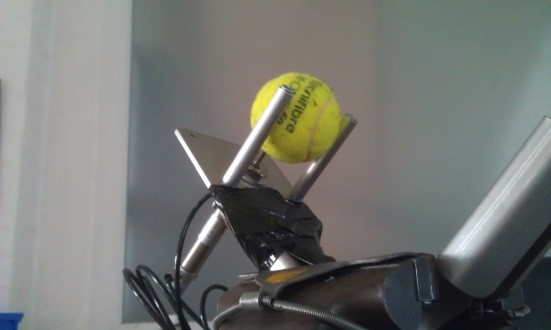
\includegraphics[width=0.8\textwidth]{Funktionstests/Bilder/PneumatikzylinderBild.jpg}
	\centering
	\caption{Funktionsmuster Pneumatikzylinder} 
\label{abb:PneumatikzylinderBild}
\end{figure}